\chapter*{Data Representation}

In this chapter we want to introduce our main ideology behind the Data Representation. Our main goal is to determine different motions for different given scenarios, while keeping it as simplified as possible.
The main idea behind simplifying the decisions, is motivated through given situations in which the robot would be to dependent on multiple parameters in order to suceed and execute its motion.
By simplifying these scenarios the robots decision will rely on less parameters thus the succes rate on making decisions will rise.

\section*{The Knowledgebase}
We designed a Ontology in which we illustrated our needed classes. 
The Knowledgebase is divided upon the superclasses Ingredient, Tools, Tasks, Motions and Container.
\begin{figure}[H]
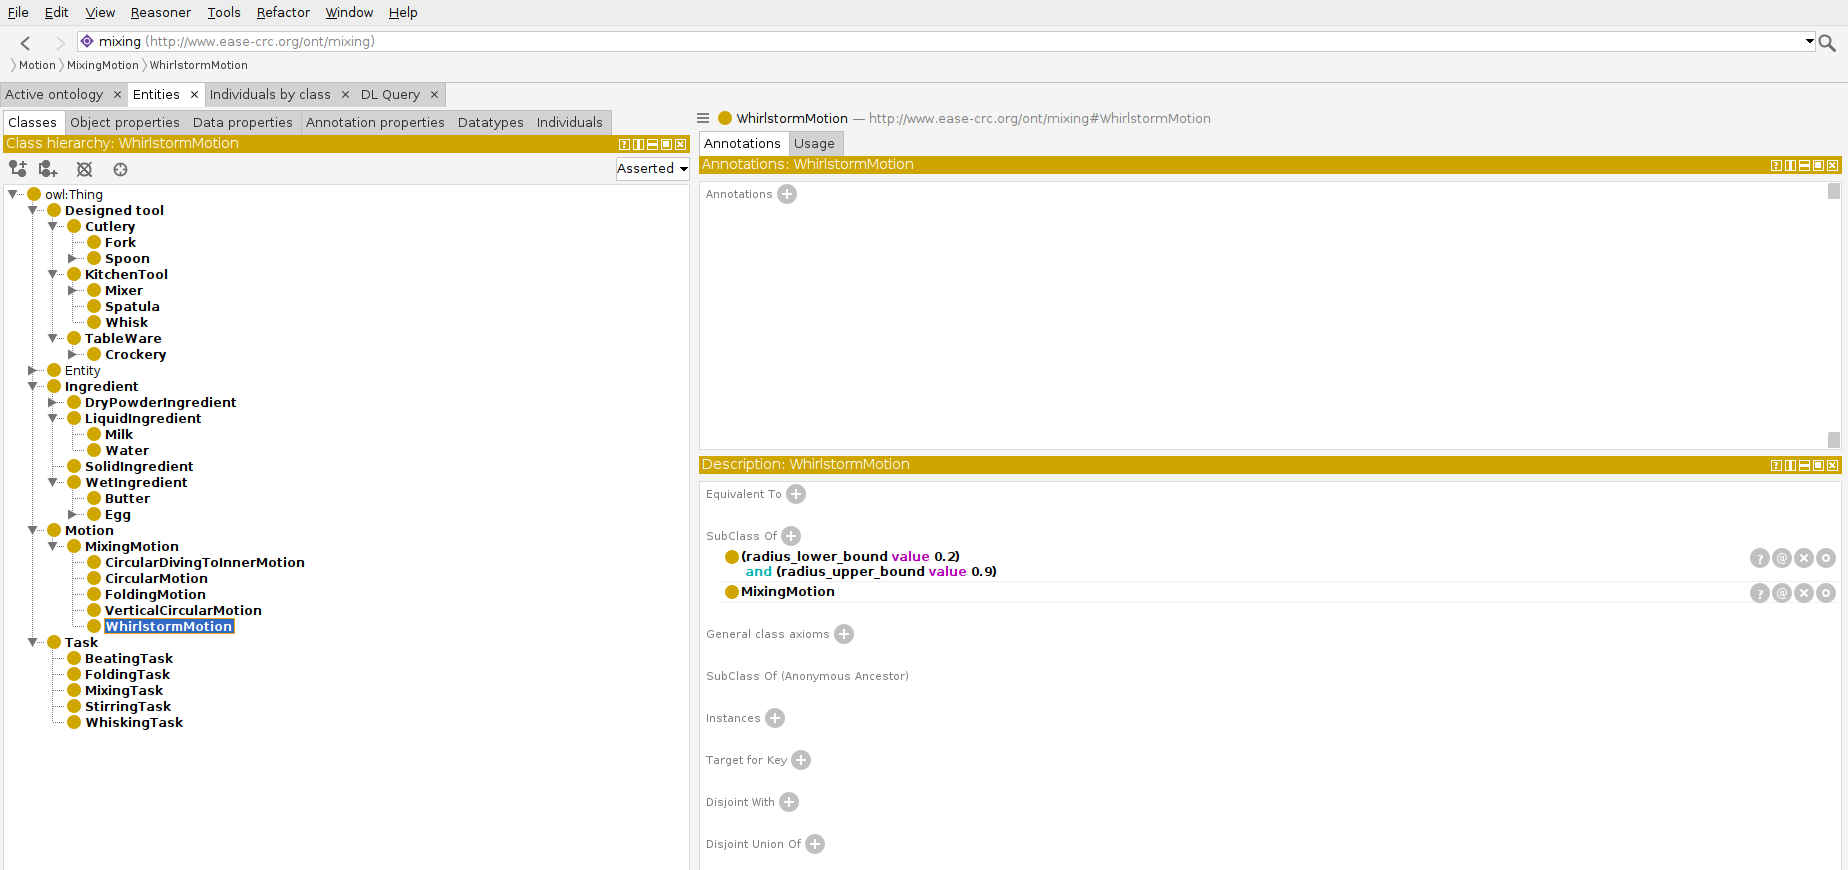
\includegraphics[scale=0.3]{Graphics/Ontology.png}
\end{figure}
\subsection*{Ingredients}
The Ingredient has 4 subclasses: WetIngredients, SolidIngredients, LiquidIngredients and DryPowderIngredients.
The WetIngredients are all the ingredients that can not be considered liquids but also not considered dry and solid, like (melted) butter or eggyolk. 
Liquid ingredients consists of liquids such as water and milk. Powder ingredients are the ingredients which are dry but also consists of small particles like sugar, salt and flour.
Last we have the solid ingredients which consists of ingredients with solid material like vegetables, fruits and meat.

\subsection*{Tools and containers}
The tools can be also divided in multiple categories. Cutlery consists of Fork and Spoon, while Spoon also has subclasses like a wooden spoon and tea spoon.
Then we have kitchen tools where we can find different types of mixers and whisks. Last we got the superclass Crockery in which our containers we will be saved, like different bowls, pot and mugs.

\subsection*{Tasks}
Different Tasks will be saved under the Task superclass. The tasks consists of Mixing, which can be regarded as the umbrela term of all tasks, Stirring which is mostly a task that includes a circular motion, Beating will be mostly used in context with eggs and other wet ingredients, Folding which represents a gentle type of mixing and the last task is whisking which is similar to the beating task.
While some of these tasks can be regarded as deterministic when considering the motion decision, like the folding task will always rely on a folding motion, we discovered that the task itself is not as ausschlaggebend, but in combination with the ingredients, one can decide upon a better motion decision. 

\subsection*{Motions}
The motions are necessary for the robotic system to know what has to be done?. The motions are inferred from Rules that regards a task component, combined with ingredients.
The motion also contain parameters, which should determine the moving space available for the robotic system. As in the mixing world, most of the container have a circular formed base, our motions are defined with a radius.
The most important parameters are:
\begin{itemize}
    \item Radius Lower Bound: This parameter describes the smallest possible radius for a motion. For example if the used container is a bowl, that has a radius of 10 cm, a radius lower bound of 0.1 would imply that the smallest possible radius on which the robot can perform its motion is 1 cm.
    \item Radius Upper Bound: Similar to the radius lower bound, the upper bound determines the maximum radius on which the robot can execute motions.
\end{itemize}
Our implemented motions are:
\begin{itemize}
    \item Circular Motion: A circular motion is a motion defined on a circular with a constant radius. This motion basically sets the 2 parameters radius upper bound and radius lower bound on the same value.  \newline HIER BILD
    \item Whirlstorm Motion: The Whirlstorm motion covers multiple parts of the container, the motion starts on the center of the container and increments its radius until it reaches the radius upper bound parameter, before turning back to the center. \newline HIER BILD
    \item Folding Motion: Folding is a special motion which is mostly used in the context of the folding task. The motion's goal is to mix the ingredients gently without overmixing the mixture. The motion starts on a point on the circle with the radius of the upper bound parameter, from there the motion draws a straight line to the middle point of the container, then getting back to the start point, next the tool will be moved 90 degrees on the defined circle and it moves back to the middle, this motion is repeteadet 4 times, and then you move the tool 20 degrees to cover all of the ingredients before starting the cycle again. \newline HIER BILD
    \item Vertical Circular Motion: The last motion can also be seen as the most difficult one. The main idea of this motion is to `wildly` mix the ingredients. Beschreibung fehlt, Bild hier rein.
\end{itemize}

\section*{Rules}
In order to infer the right motion based on the ingredients and task input, rules have to be defined. This rules are written in SWRL, which was presented in the USEDLIBRARIES section. In this section we want to illustrate the inference on a high level, while the implementation of it will be shown in the implementation chapter. 
The rules can be thoguht was if conditions, which will then result in a motion. For example, if we regard the combination of the task Mixing and the ingredient type liquid, we infer the motion Whirlstormmotion. This can be done for every task and ingredient combination. 
The inference can be illustrated with decision trees which will be shown in the next images for every task and ingredient type combination available. 
Hier die decision trees?.

\subsection*{Mixing}
\begin{figure}[H]
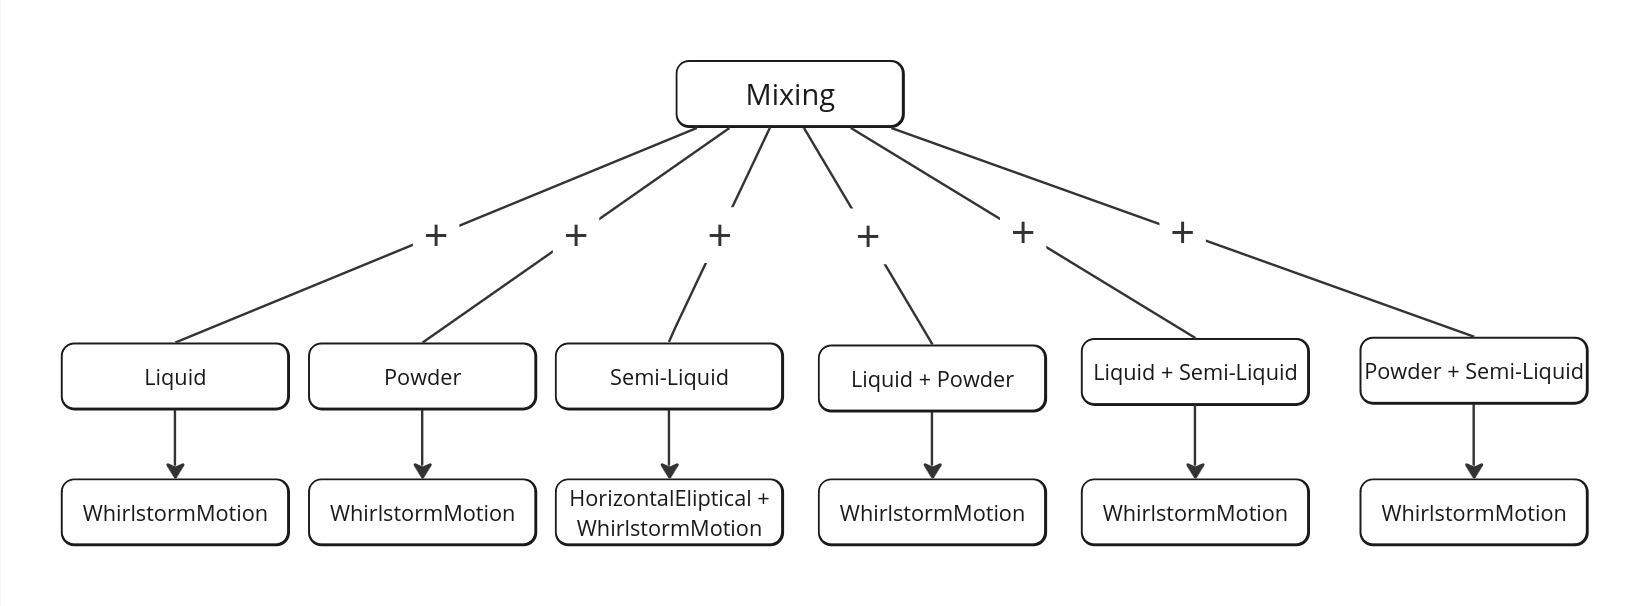
\includegraphics[scale=0.18]{Graphics/MixingDecisionTree.jpg}
\end{figure}
\textbf{Definition:} In the context of baking or cooking, a mixing task refers to the process of combining multiple ingredients thoroughly to create a homogeneous mixture. The goal is to distribute the ingredients evenly, ensuring that each component contributes to the overall texture, flavor, and consistency of the final dish or baked good. Mixing is a fundamental step in many recipes and is essential for achieving a balanced and cohesive result.


Wie man anhand der Abbildung erkennen kann, kann die Mixing Task hauptsächlich auf die Whirlstormmotion abgebildet werden. Dies wundert letzendlich nicht, wenn man sich die Definion anschaut, denn diese Motion führt dazu, dass alle Zutaten in dem Behälter gleichmäßig verteilt werden.

\subsection*{Stirring}
\begin{figure}[H]
    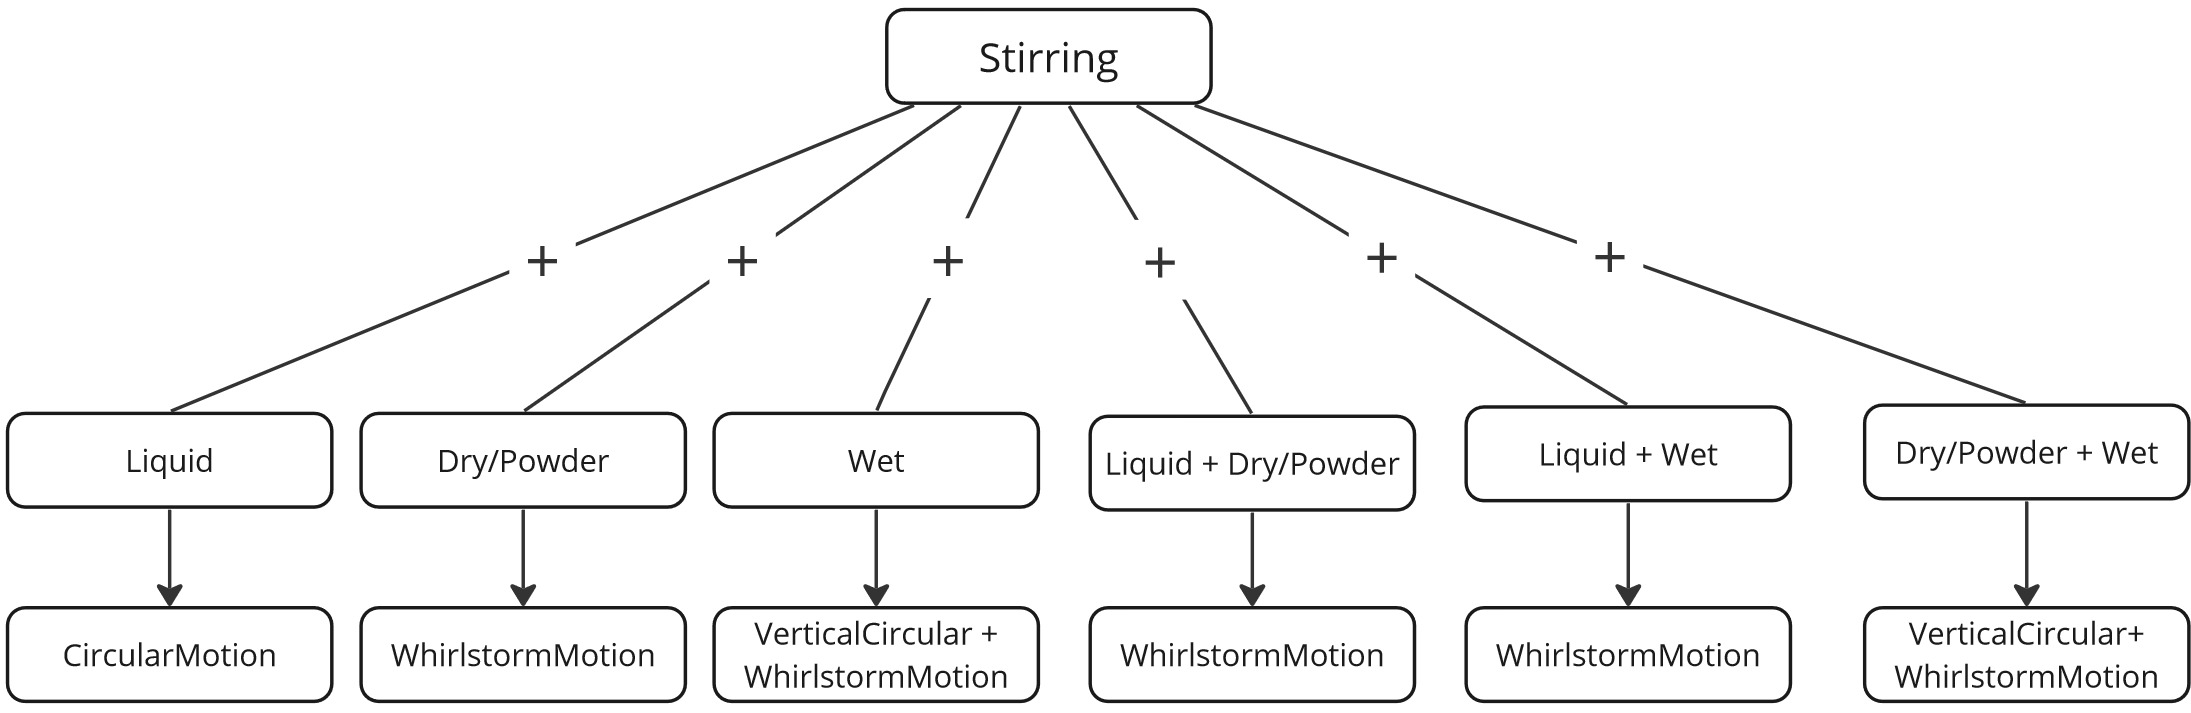
\includegraphics[scale=0.18]{Graphics/StirringDeisionTree.jpg}
    \end{figure}
\textbf{Definition:}
In the context of baking or cooking, a stirring task involves using a utensil, such as a spoon, spatula, or whisk, to agitate and circulate the ingredients within a mixture. The purpose of stirring is to achieve a uniform distribution of ingredients

Im Vergleich zu Mixing bildet die Stirring Task abhängig von den Zutaten auf eine breitere Anzahl von Motions ab. Neben der Whirlstormmotion wird hier zum ersten Mal die CircularMotion genutzt. Diese ist besonders wichtig in Anbetracht der Stirring Task mit dem Ingredienttyp Liquid, da man nicht möchte, wie bei der Whirlstormmotion der Fall wäre, dass die Zutaten "aufgerührt" werden, sondern ledigilich umgerührt.

\subsection*{Beating}
\begin{figure}[H]
    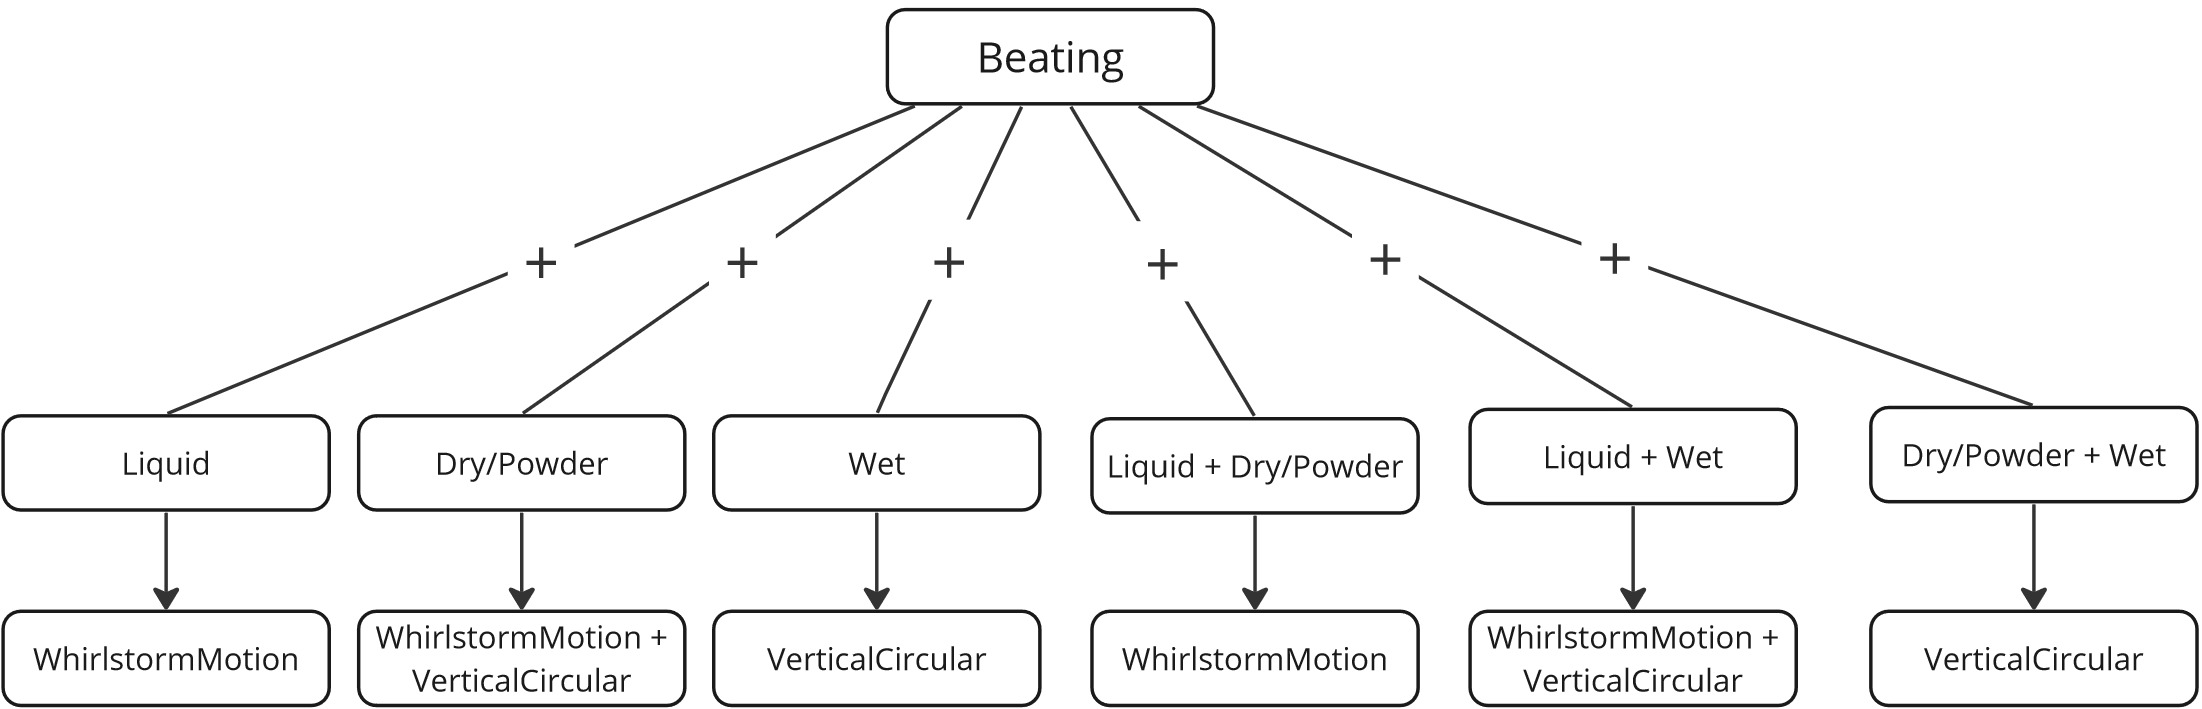
\includegraphics[scale=0.18]{Graphics/BeatingDecisionTree.jpg}
    \end{figure}
\textbf{Definition:}
In the context of baking and cooking, a "beating" task refers to the process of vigorously stirring or mixing ingredients to achieve a specific texture or consistency. Beating is often done to incorporate air into the mixture, create smooth and uniform blends, or alter the physical properties of certain ingredients.

Neben der WhirlstormMotion prädominiert hier auch die VerticalCircular Motion, dies ist auch aus der Definition abzuleiten, da diese Motion eine willkürliche Art des Mixen erfordert, worauf die VerticalCircular Motion passt.

\subsection*{Whisking}
\begin{figure}[H]
    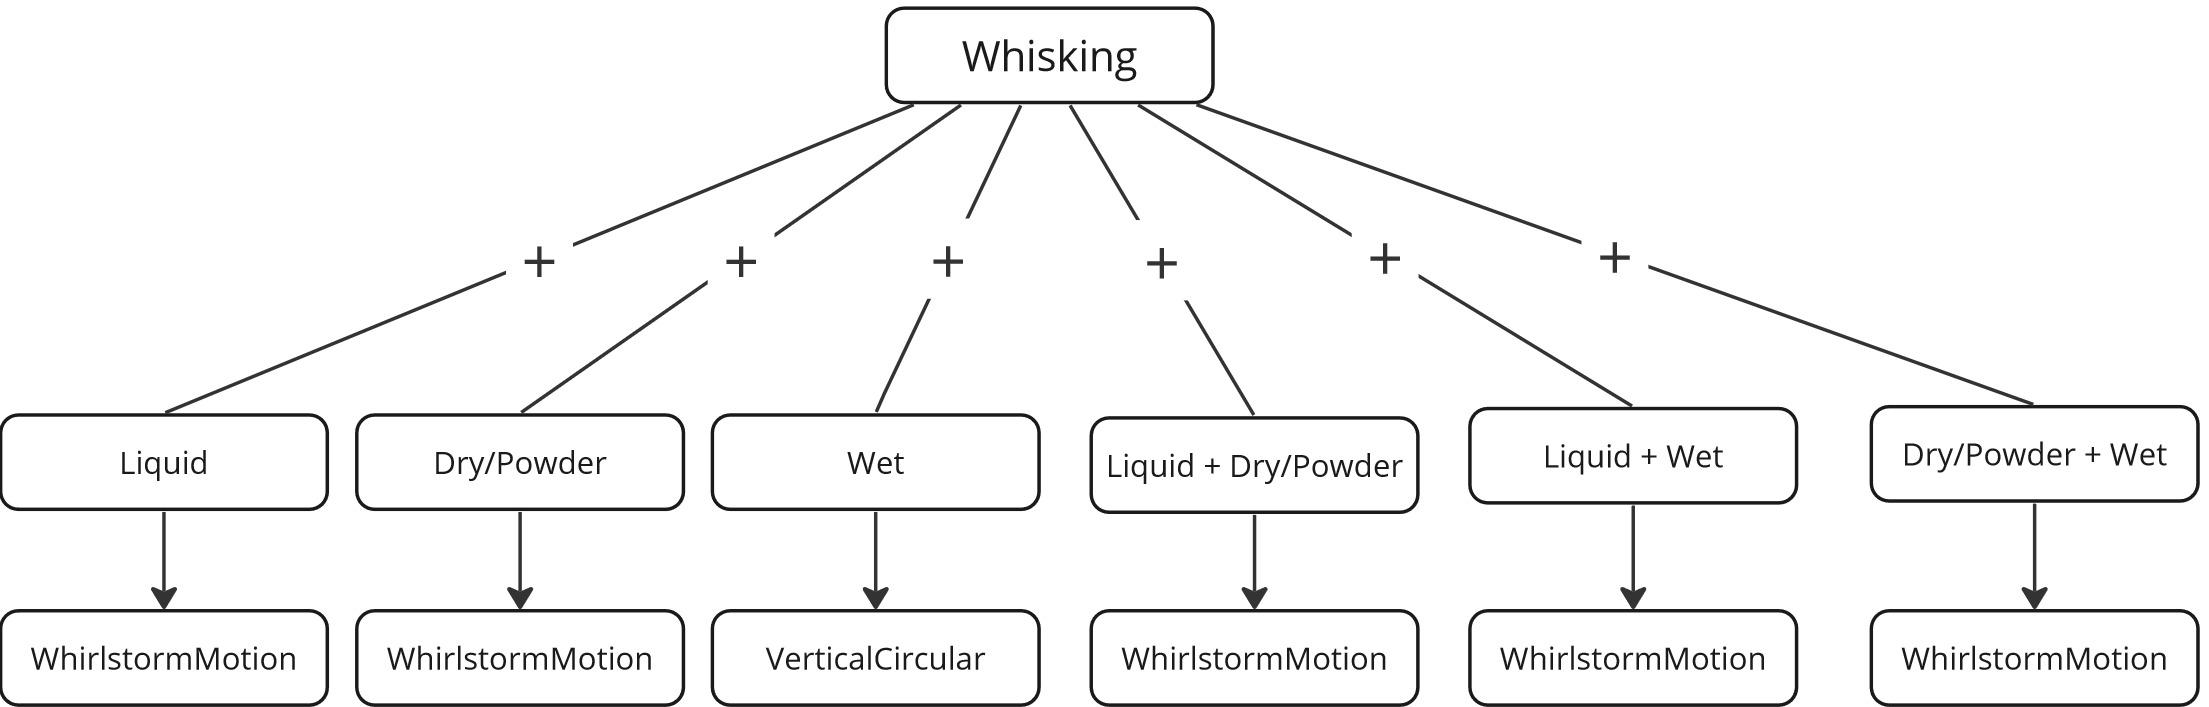
\includegraphics[scale=0.18]{Graphics/WhiskingDecisionTree.jpg}
    \end{figure}
\textbf{Definion:}In the context of baking and cooking, a "whisking" task involves using a kitchen utensil called a whisk to mix, blend, or beat ingredients. A whisk typically consists of wire loops or a coil attached to a handle, and it is designed to incorporate air into mixtures, break up clumps, and create a smooth and uniform texture.

\subsection*{Folding}
\begin{figure}[H]
    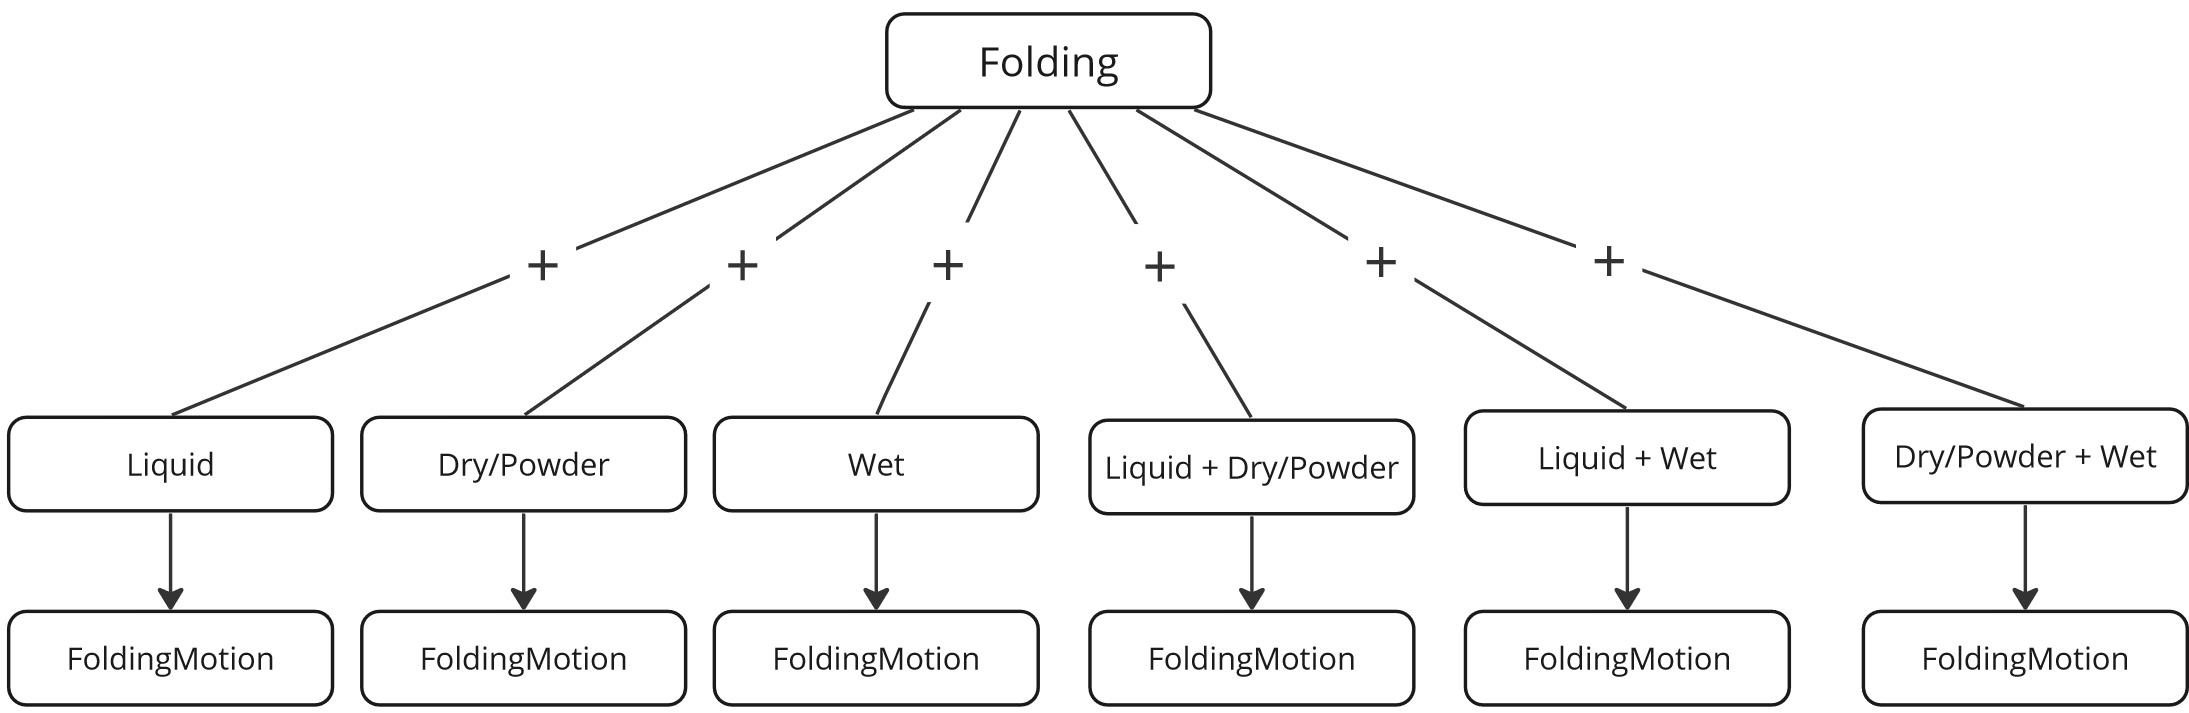
\includegraphics[scale=0.18]{Graphics/FoldingDecisionTree.jpg}
    \end{figure}
\textbf{Definition:}
In the context of baking and cooking, a "folding" task refers to a gentle mixing technique used to incorporate ingredients without deflating or destroying the air bubbles that have been created. Folding is often employed when combining a lighter mixture (such as whipped cream or beaten egg whites) with a denser one (such as a batter or a heavier mixture). The goal is to maintain the desired texture, lightness, or fluffiness in the final dish.

Theoretisch müssten wir die Folding Task nicht grafisch darstellen, da jede Task und Ingredients Kombination auf eine einzige Motion abbildet, die FoldingMotion. Die Grafik wurde trotzdem der vervollstädnigkeitshalber eingefügt.
Die FoldingTask erfodert eine spezifische Bewegung, die die Luft in der Mixtur nicht entfernt, wobei jede andere Bewegung scheitern würde.

\section*{How to expand the Knowledgebase}